%set the master document for easy compilation
%!TEX root = ../D3_5_3.tex

\section{F2.12: manageTIU\_input}\label{s:F2.12}


\subsection{Component Requirements}

\begin{longtable}{p{.25\textwidth}p{.7\textwidth}}
\toprule
Component name			& manageTIU\_input \\
\midrule
Link to SCADE model		& {\footnotesize \url{https://github.com/openETCS/modeling/tree/master/model/Scade/System/ObuFunctions/manageData/manageTIU}} \\
\midrule
SCADE designer			& Bernd Hekele, DB Netz AG \\
\midrule
Description				& This component manages the incoming messages and information that are received from the Train Interface Unit (TIU), e.g. cab status information.
% This includes determining the position of the direction controller and whether the cab desk is open or close. 
%2-Engine control. An interface is included to cut the traction power. This is used when the ETCS onboard equipment is applying either the service or emergency brakes and needs to ensure that tractive effort is no longer being applied
\\
\midrule
Input documents	& 
Alstom API\newline
Subset-034\\
\midrule
Safety integrity level		& 4 \\
\midrule
Time constraints		& n/a
 \\
\midrule
API requirements 		& n/a\\
\bottomrule
\end{longtable}


\subsection{Interface}

An overview of the interface of component manageTIU\_input is shown in Figure~\ref{f:manageTIUInput}.  For the description of inputs and outputs we refer to the SCADE Suite model (cf. link above)  respectively the SCADE generated documentation.
%The inputs and outputs are described in detail in Section~\ref{s:manageTIUInput_inputs} respectively \ref{s:manageTIUInput_outputs}. 
Subcomponents are described in Section~\ref{s:manageTIUInput_subcomponents}.

\begin{figure}[H]
\center
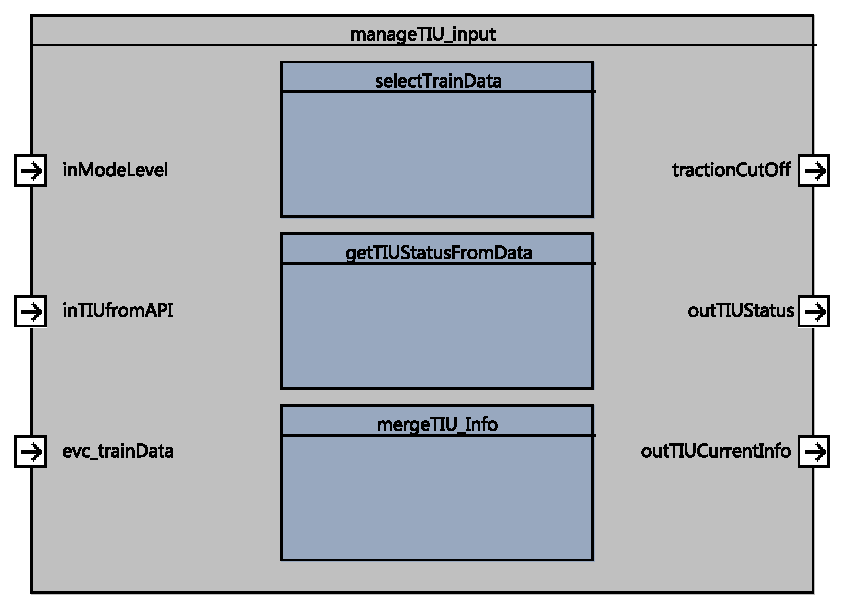
\includegraphics[width=.7\textwidth]{images/F2_12_manageTIU_input.pdf}
\caption{manageTIU\_input SysML diagram.}\label{f:manageTIUInput}
\end{figure}

%
%\subsubsection{Inputs}\label{s:manageTIUInput_inputs}
%
%\paragraph{[Input 1 name]}
%
%\begin{longtable}{p{.25\textwidth}p{.7\textwidth}}
%\toprule
%Input name				& [Name of the input] \\
%\midrule
%Description				& [Brief description of the input] \\
%\midrule
%Source					& [Name of the source component] \\ 
%\midrule
%Type					& [Type of the input] \\
%\midrule
%Valid range of values	& [Complete list of valid values] \\
%\midrule
%Behaviour when value is at boundary	& [Description of components behaviour when input value is at boundary] \\
%\midrule
%Behaviour for values out of valid range	& [Description of components behaviour when input value is out of valid range] \\
%\midrule
%Behaviour when value is erroneous, absent or unwanted (i.e. spurious) & [Description of components behaviour when value is erroneous, absent or unwanted (i.e. spurious)] \\
%\bottomrule
%\end{longtable}
%
%
%\paragraph{[Input 2 name]}
%
%\begin{longtable}{p{.25\textwidth}p{.7\textwidth}}
%\toprule
%Input name				& [Name of the input] \\
%\midrule
%Description				& [Brief description of the input] \\
%\midrule
%Source					& [Name of the source component] \\ 
%\midrule
%Type					& [Type of the input] \\
%\midrule
%Valid range of values	& [Complete list of valid values] \\
%\midrule
%Behaviour when value is at boundary	& [Description of components behaviour when input value is at boundary] \\
%\midrule
%Behaviour for values out of valid range	& [Description of components behaviour when input value is out of valid range] \\
%\midrule
%Behaviour when value is erroneous, absent or unwanted (i.e. spurious) & [Description of components behaviour when value is erroneous, absent or unwanted (i.e. spurious)] \\
%\bottomrule
%\end{longtable}
%
%
%\subsubsection{Outputs}\label{s:manageTIUInput_outputs}
%
%\paragraph{[Output 1 name]}
%
%\begin{longtable}{p{.25\textwidth}p{.7\textwidth}}
%\toprule
%Output name				& [Name of the output] \\
%\midrule
%Description				& [Brief description of the output] \\
%\midrule
%Destination				& [Name of the destination component(s)] \\ 
%\midrule
%Type					& [Type of the output] \\
%\midrule
%Valid range of values	& [Complete list of valid values] \\
%\midrule
%Behaviour when value is at boundary	& [Description of components behaviour when output value is at boundary] \\
%\midrule
%Behaviour for values out of valid range	& [Description of components behaviour when output value is out of valid range] \\
%\midrule
%Behaviour when value is erroneous, absent or unwanted (i.e. spurious) & [Description of components behaviour when value is erroneous, absent or unwanted (i.e. spurious)] \\
%\bottomrule
%\end{longtable}
%
%
%\paragraph{[Output 2 name]}
%
%\begin{longtable}{p{.25\textwidth}p{.7\textwidth}}
%\toprule
%Output name				& [Name of the output] \\
%\midrule
%Description				& [Brief description of the output] \\
%\midrule
%Destination				& [Name of the destination component(s)] \\ 
%\midrule
%Type					& [Type of the output] \\
%\midrule
%Valid range of values	& [Complete list of valid values] \\
%\midrule
%Behaviour when value is at boundary	& [Description of components behaviour when output value is at boundary] \\
%\midrule
%Behaviour for values out of valid range	& [Description of components behaviour when output value is out of valid range] \\
%\midrule
%Behaviour when value is erroneous, absent or unwanted (i.e. spurious) & [Description of components behaviour when value is erroneous, absent or unwanted (i.e. spurious)] \\
%\bottomrule
%\end{longtable}

\subsection{Subcomponents}\label{s:manageTIUInput_subcomponents}

The subcomponents of ManageTIUInput are not documented in this version of the architecture and design description document.
%\subsubsection{mergeTIU\_Info}
%%set the master document for easy compilation
%!TEX root = ../D3_5_3.tex

\paragraph{Component Requirements}

\begin{longtable}{p{.25\textwidth}p{.7\textwidth}}
\toprule
Component name			& mergeTIU\_Info \\
\midrule
Link to SCADE model		& {\footnotesize \url{https://github.com/openETCS/modeling/tree/master/model/Scade/System/ObuFunctions/manageData/manageTIU}} \\
\midrule
SCADE designer			& Bernd Hekele, DB Netz AG \\
\midrule
Description				&  This interface is included to cut the traction power. This is used when the ETCS onboard equipment is applying either the service or emergency brakes and needs to ensure that tractive effort is no longer being applied \\
\midrule
Input documents	& 
Alstom API\newline
Subset-034\\
\midrule
Safety integrity level	& 4 \\
\midrule
Time constraints		&\todo[inline]{section and corresponding subsections have to be completed} \\
\midrule
API requirements 		&\todo[inline]{section and corresponding subsections have to be completed} \\
\bottomrule
\end{longtable}


\paragraph{Interface}

For an overview of the interface of this internal component we refer to the SCADE model (cf.~link above) respectively the SCADE generated documentation.

%\subsubsection{getTIUStatusFromData}
%%set the master document for easy compilation
%!TEX root = ../D3_5_3.tex

\paragraph{Component Requirements}

\begin{longtable}{p{.25\textwidth}p{.7\textwidth}}
\toprule
Component name			& getTIUStatusFromData \\
\midrule
Link to SCADE model		& {\footnotesize \url{https://github.com/openETCS/modeling/tree/master/model/Scade/System/ObuFunctions/manageData/manageTIU}} \\
\midrule
SCADE designer			& Bernd Hekele, DB Netz AG \\
\midrule
Description				& [Brief description of functionality] \\
\midrule
Input documents	& 
Alstom API\newline
Subset-034\\
\midrule
Safety integrity level	& 4 \\
\midrule
Time constraints		&\todo[inline]{section and corresponding subsections have to be completed} \\
\midrule
API requirements 		&\todo[inline]{section and corresponding subsections have to be completed} \\
\bottomrule
\end{longtable}


\paragraph{Interface}

For an overview of the interface of this internal component we refer to the SCADE model (cf.~link above) respectively the SCADE generated documentation.